\section{Recommendations con i Grafi}
Negli ultimi anni, i sistemi di raccomandazione hanno assunto un ruolo centrale in numerosi ambiti applicativi, dall’e-commerce ai social media, dallo streaming musicale ai motori di ricerca. Tradizionalmente, questi sistemi si basano su approcci collaborativi o contenutistici; tuttavia, l'utilizzo della rappresentazione a grafo ha aperto nuove possibilità in termini di espressività, scalabilità e qualità delle raccomandazioni.
\\
Un grafo permette di modellare in modo naturale le relazioni complesse tra utenti, item (prodotti, film, post, ecc.) e altri fattori contestuali, come tag, categorie o interazioni temporali. In questo contesto, i sistemi di recommendation basati su grafi sfruttano la struttura topologica per propagare preferenze, misurare somiglianze e generare suggerimenti più pertinenti anche in scenari con dati scarsi o altamente dinamici.

\paragraph{Definizione} Il termine sistema di raccomandazione (RS) si riferisce a tutti gli strumenti software e le tecniche che, utilizzando le conoscenze che possono raccogliere sugli utenti e sugli elementi in questione, suggeriscono elementi che potrebbero essere di interesse per un particolare utente. Il motivo principale per cui questo sistema viene implementato é migliorare l'esperienza utente. 

\subsubsection*{Content Based Recommendation Systems (CBRS)}
Sono sistemi che sfruttano le descrizioni di user e items per costruire delle rappresentazioni che abbiano una base semantica: collegare cose simili anche per descrizione potenzia la capacitá di fare collegamenti utili. Processo base:
\begin{itemize}
    \item Abbinando gli attributi del profilo utente target con gli attributi degli elementi per trovare elementi simili a ciò che l'utente ha apprezzato in passato, il risultato è un punteggio di pertinenza che prevede il livello di interesse dell'utente target per quegli elementi.
    \item In genere, gli attributi per descrivere un elemento sono caratteristiche estratte dai metadati associati a quell'elemento o caratteristiche testuali in qualche modo correlate all'elemento: descrizioni, commenti, parole chiave e così via.
    \item I CBRS utilizzano questi elementi ricchi di contenuto per effettuare confronti o dedurre gli interessi di un utente in base all'elenco di elementi con cui ha interagito.
\end{itemize}
\paragraph{High-Level Architecture} Tre componenti di base nell'architettura di un CBRS:
\\
\begin{figure}[th]
    \centering
    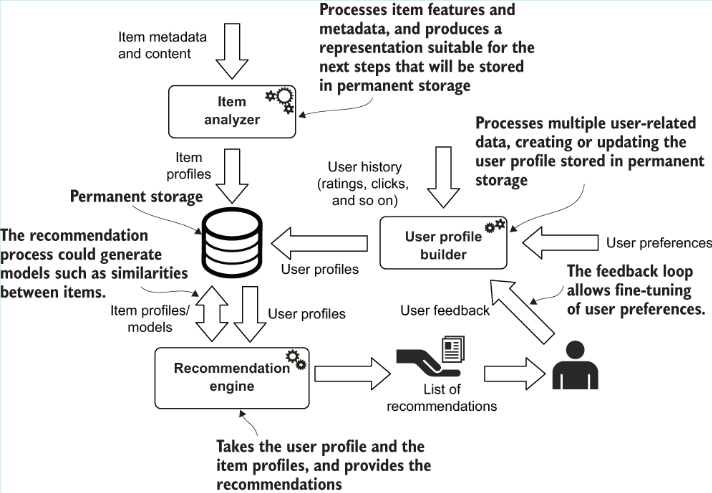
\includegraphics[width=0.4\linewidth]{RecommendationsGraph//img/cbrs.png}
\end{figure}
\\
\begin{itemize}
    \item \textbf{Item Analyser:} Estrarre o identificare le caratteristiche rilevanti (chiamate anche proprietà o attributi) e rappresentare gli elementi: prende come input il contenuto dell'elemento (il contenuto di un libro o la descrizione di un prodotto) e le metainformazioni (l'autore del libro, gli attori di un film...) da più di 1 fonte di informazioni e le converte in un modello di elemento che viene utilizzato in seguito per fornire raccomandazioni.
    \item \textbf{User Profile Builder:} Questo processo raccoglie dati rappresentativi delle preferenze dell'utente e ne deduce i profili utente, interrogando gli utenti sui loro interessi o raccogliendo feedback impliciti osservando e memorizzando il comportamento dell'utente. Il risultato è un modello, in particolare un modello grafico, che rappresenta l'interesse dell'utente per un elemento, una caratteristica dell'elemento o entrambi.
    \item \textbf{Recommendation Engine:} Sfrutta i profili utente e le rappresentazioni degli elementi per suggerire elementi pertinenti abbinando gli interessi dell'utente alle caratteristiche dell'elemento. In questa fase, viene creato un modello predittivo che viene utilizzato per creare un punteggio di pertinenza per ciascun elemento per ciascun utente. Questo punteggio viene utilizzato per classificare e ordinare gli elementi da suggerire all'utente.
\end{itemize}
In un CBRS, esistono diversi metodi per raccogliere e modellare i profili utente. Il modello di progettazione selezionato varierà a seconda di come vengono raccolte le preferenze (implicitamente o esplicitamente) e del tipo di strategia di filtraggio o approccio di raccomandazione. Un modo semplice per raccogliere le preferenze dell'utente è chiedere direttamente all'utente. L'utente potrebbe esprimere interesse per generi o parole chiave specifici, o per attori o registi specifici. Da una prospettiva di alto livello, lo scopo del profilo utente e del modello definito è quello di aiutare il motore di raccomandazione ad assegnare un punteggio a ciascun elemento o caratteristica dell'elemento. Il punteggio aiuta a classificare gli elementi suggeriti all'utente specifico, ordinati dal più alto al più basso. Per questo motivo, i sistemi di raccomandazione appartengono all'area del machine learning chiamata "learning to rank".
\newpage


\subsection{Collaborative Filtering}
Un'alternativa al filtraggio dei contenuti si basa esclusivamente sul comportamento passato degli utenti, come transazioni precedenti o valutazioni degli articoli, o sulle opinioni di una community di utenti esistente, per prevedere quali articoli saranno più probabilmente apprezzati o interessati agli utenti, senza richiedere la creazione di profili espliciti sia per gli articoli che per gli utenti in base alle caratteristiche degli articoli. Questo approccio è noto come \textbf{Collaborative Filtering}, un termine coniato dagli sviluppatori di Tapestry [Goldberg et al., 1992], il primo sistema di raccomandazione. Il filtraggio collaborativo analizza le relazioni tra gli utenti e le interdipendenze tra gli articoli per prevedere nuove associazioni utente-articolo.

\begin{figure}[th]
    \centering
    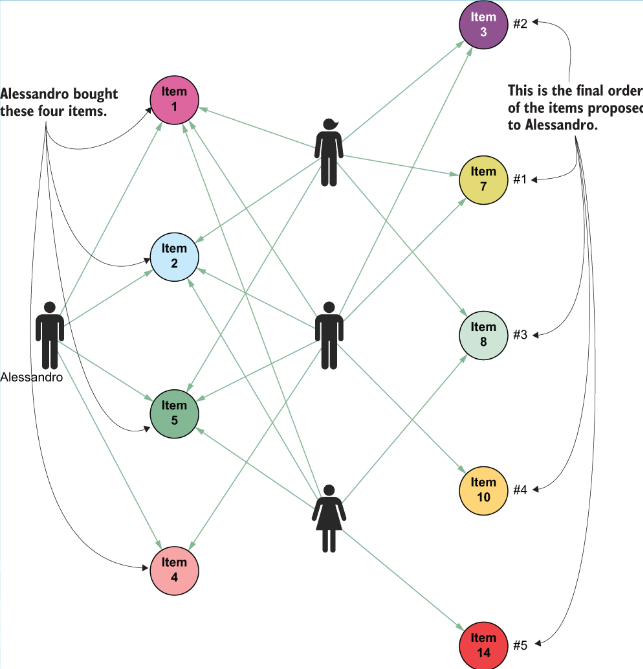
\includegraphics[width=0.45\linewidth]{RecommendationsGraph//img/collaborativefiltering.png}
\end{figure}

\paragraph{Vantaggi} 
\begin{itemize}
    \item É domain free
    \item Non ha bisogno di nessun dettaglio sugli items
    \item Puó essere applicato ad una grande varietá di casi, e puó trovare informazioni rilevanti difficili da vedere con content filtering
\end{itemize}

\paragraph{Svantaggi}
\begin{itemize}
    \item Il problema dell'avvio a freddo è dovuto all'incapacità di fornire raccomandazioni ragionevoli (in termini di accuratezza) per nuovi elementi e utenti o quando sono disponibili dati di interazione limitati. Esistono tuttavia meccanismi che attenuano l'effetto del problema dell'avvio a freddo utilizzando diversi algoritmi, come l'approccio del grafo o altre fonti di conoscenza, come i social network.
\end{itemize}
Quindi per risolvere il problema del cold start, un primo approccio potrebbe essere quello di valorizzare informazioni aggiuntive sull'utente, come il gender, educazione, interessi... questo aiuterebbe nella sua classificazione (quindi aggiungere informazioni per migliorare la profilazione); il secondo approccio é creare sistemi per raccomandazioni ibridi, che uniscono diversi approcci in un singolo meccanismo di predizione.

\paragraph{User-based approach} Se due utenti avevano gusti simili in passato, avranno gusti simili anche in futuro. Le preferenze degli utenti rimangono stabili e coerenti nel tempo. Sulla base di questa assunzione, possono succedere due cose:
\begin{itemize}
    \item Interazione tra users e items non ha peso. Questo caso é chiamato modello booleano o binario. 
       \[
    score(a,b) = \frac{1}{|KNN(a)|} \times \sum_{b\in KNN(a)} r_{b,p}
    \]
    \item Interazione pesata. Con una formula che prevede i ratings che un user assegnerá ad un item. 
    \[
    pred(a,p) = \frac{\sum_{b\in KNN(a)} sim(a,b)}{\sum_{b\in KNN(a)} |sim (a,b)|} \times r_{b,p}
    \]
\end{itemize}
Quello che si vuole fare è una media pesata dei rating degli utenti simili.

\paragraph{Item-based approach} Questo tipo di approccio permette il calcolo in real-time. Ovviamente l'idea alla base é quella di usare similaritá tra gli elementi e cercare elementi simili piuttosto che tra gli users. La formula per prevedere il rating di un elemento non ancora presente in un dataset é: 
\[
    pred(a,p) = \frac{\sum_{q\in ratedItem(a)} (sim(p,q) \times r_{a, q} \times |KNN(q) \cap \{ p \}|)}{\sum_{q\in ratedItem(a)} (sim(p,q) \times |KNN(q) \cap \{ p \}|)}
\]
Dove $q$, simboleggia ogni elemento considerato e valutato dall'user $a$. Per ogni $q$, moltiplica tre valori: 
\begin{itemize}
    \item la similaritá tra $q$ e il target product $p$,
    \item il rating assegnato a $q$ dall'user,
    \item $|KNN(q) \cap \{ p \}|)$ é 1 se $p$ si trova nel set dei NN, altrimenti é 0
\end{itemize}
Il denominatore normalizza il valore per non eccedere nella valutazione del rating. 

\subsubsection*{Summary}
Gli aspetti e i vantaggi principali dell'approccio basato su grafi ai motori di raccomandazione per collaborative filtering implementati con metodi NN sono i seguenti:
\begin{itemize}
    \item Il dataset Utente-Elemento può essere facilmente rappresentato come un grafo bipartito, in cui il peso di ciascuna coppia utente-elemento è rappresentato come una proprietà opzionale della relazione.
    \item La rappresentazione a grafo bipartito del dataset Utente-Elemento non solo ha il vantaggio di consentire di memorizzare solo le informazioni rilevanti, evitando di sprecare memoria memorizzando zeri inutili, come nella rappresentazione a matrice, ma anche di velocizzare l'accesso durante la creazione del modello concentrandosi solo sui vicini potenzialmente rilevanti.
    \item È possibile estrarre diverse rappresentazioni vettoriali sia per gli elementi che per gli utenti dallo stesso modello di grafo.
    \item Il modello risultante, costituito da somiglianze tra utenti o elementi o entrambi, può essere rappresentato naturalmente come nuove relazioni che collegano utenti ed elementi. I nuovi grafi risultanti sono le reti del vicino più prossimo (k-NN).
    \item L'algoritmo, basato sul calcolo della similarity, per la creazione delle reti k-NN rappresenta una delle tecniche più potenti e ampiamente adottate per la costruzione di grafi. Le reti risultanti non solo sono facili da navigare durante il processo di raccomandazione, ma contengono anche nuove conoscenze, ricavate dal dataset Utente-Elemento esistente, che possono essere utilizzate per analizzare i dati da altre prospettive, come il clustering degli elementi, la segmentazione dei clienti e così via.
    \item Una tecnica ampiamente adottata per risolvere il problema della scarsità di dati e il problema dell'avvio a freddo si basa sulla rappresentazione, la navigazione e l'elaborazione dei grafi. Anche in questo scenario, è possibile combinare più algoritmi di raccomandazione in un singolo grafo e combinare la potenza di più approcci per fornire raccomandazioni.
\end{itemize} 

\subsection{Fraud Detection}
Alcune delle tecniche di rilevamento delle frodi che vedremo provengono dal campo più generico del rilevamento di anomalie o valori anomali. Un'anomalia o un valore anomalo si riferisce a un data point che differisce significativamente dagli altri. Nel contesto delle frodi, questo si verifica in comportamenti (come le transazioni) che si discostano dal comportamento abituale di un individuo, il che può essere un indicatore di attività fraudolenta. Oltre a rivelare comportamenti sospetti o anomali in ambito finanziario, il rilevamento delle anomalie è fondamentale per individuare eventi rari come epidemie di malattie rare o effetti collaterali in ambito medico, con applicazioni vitali nella diagnosi medica. Un'altra applicazione del rilevamento delle anomalie è la pulizia dei dati, ovvero la rimozione di valori errati o rumore dai dati come fase di pre-elaborazione per consentire l'apprendimento di modelli più accurati dei dati.
\begin{quote}
    Fraud is an uncommon, well-considered, time-evolving, caref
ully organized and imperceptibly concealed crime that appear
s in many different types and forms.
\end{quote}
Quindi come si fa \textbf{Fraud detection?} Il rilevamento delle frodi si riferisce alla capacità di riconoscere o scoprire le frodi. Entra in gioco quando la prevenzione delle frodi fallisce, ma poiché non è sempre ovvio quando ciò accade, è necessario utilizzare costantemente misure di rilevamento delle frodi. Possiamo fare del nostro meglio per prevenire le frodi sulle carte di credito, ma se i dati di una carta vengono rubati, dobbiamo essere in grado di rilevare l'uso fraudolento il prima possibile. Quando parliamo di \textbf{Fraud prevention} facciamo invece riferimento a tutte quelle contromisure volte a limitare l'efficacia delle frodi. 
\subsubsection*{Rule-based engine}
Un \textbf{rule-based engine} per la \textbf{fraud detection} è un sistema che rileva comportamenti sospetti applicando un insieme di \emph{regole predefinite}. Queste regole sono definite da esperti del dominio e descrivono condizioni logiche che, se soddisfatte, indicano potenziali frodi.
\\
Le regole possono essere formulate come condizioni del tipo:
\begin{itemize}
  \item Se l'importo di una transazione supera i 10.000\,€ \emph{e} proviene da un paese non abituale, allora segnalare come sospetta.
  \item Se un utente effettua più di 5 acquisti in meno di 5 minuti, allora indicare potenziale frode.
  \item Se si verificano più di 3 login falliti da un indirizzo IP sconosciuto, bloccare l'account.
\end{itemize}

Il processo tipico di un rule-based engine comprende i seguenti passi:

\begin{enumerate}
  \item \textbf{Definizione delle regole}: Le condizioni vengono scritte in pseudocodice, linguaggi SQL, DSL o strumenti specifici come \emph{Drools} o \emph{CLIPS}.
  \item \textbf{Input dei dati}: Il sistema riceve dati in tempo reale o in batch, comprendenti informazioni su utenti, transazioni, IP, dispositivi, ecc.
  \item \textbf{Applicazione delle regole}: Le regole vengono valutate sui dati ricevuti. Se una regola è soddisfatta, si può bloccare l'operazione, inviarla per revisione o aggiornarne lo score di rischio.
  \item \textbf{Logging e audit}: Ogni decisione è tracciata per garantire trasparenza e conformità.
\end{enumerate}

I \textbf{vantaggi} di questo approccio includono:
\begin{itemize}
  \item Alta \emph{spiegabilità}: è chiaro il motivo di ogni decisione.
  \item Semplicità di \emph{manutenzione} e aggiornamento.
  \item Controllo totale sul comportamento del sistema.
\end{itemize}

Tuttavia, presenta anche dei \textbf{limiti}:
\begin{itemize}
  \item \emph{Rigidità}: non si adatta a nuovi schemi di frode.
  \item Gestione complessa con molte regole.
  \item \emph{Falsi positivi} elevati se le regole sono troppo generiche.
\end{itemize}

Nelle implementazioni moderne, spesso il rule-based engine è integrato con modelli di \emph{machine learning}, formando un sistema ibrido dove:
\begin{itemize}
  \item Le regole gestiscono i casi evidenti.
  \item I modelli predittivi analizzano pattern più complessi e adattivi.
\end{itemize}

\begin{figure}[th]
    \centering
    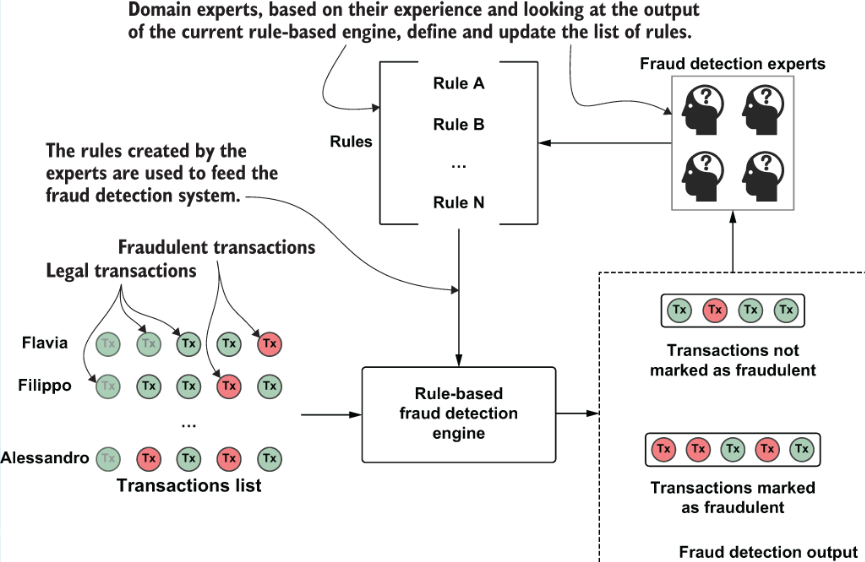
\includegraphics[width=0.62\linewidth]{RecommendationsGraph//img/frauddetectionrule.png}
\end{figure}
\newpage
\subsubsection*{Graphs for Fraud Detection}
I grafici forniscono un potente strumento di modellazione e analisi per catturare correlazioni a lungo raggio tra oggetti di dati interdipendenti, il che li rende particolarmente adatti allo scenario di lotta alle frodi. Le transazioni sui nostri conti bancari e sulle carte di credito seguono una logica legata a ciò che facciamo, a dove viviamo, a ciò che ci piace acquistare e così via. Inoltre, le frodi raramente si verificano in modo isolato: dietro ogni frode c'è un piano che prevede una preparazione, che spesso richiede la cooperazione tra più truffatori.
\begin{figure}[th]
    \centering
    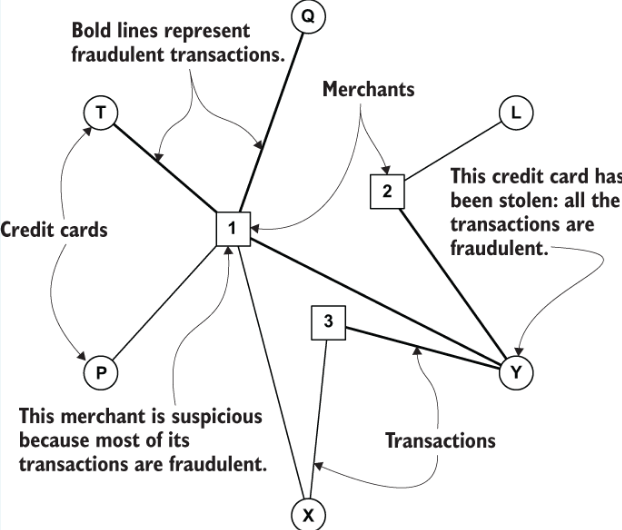
\includegraphics[width=0.5\linewidth]{RecommendationsGraph//img/graphfraud.png}
\end{figure}

\subsection{Graphs for NLP}
I motori di ricerca, i sistemi di raccomandazione e gli assistenti vocali hanno i seguenti requisiti in comune: l'uso del testo per la creazione di una knowledge base, una rappresentazione adeguata della conoscenza che memorizzi tutte le informazioni necessarie per l'ambito dell'applicazione e interazione con l'utente via natural language. L'elaborazione del linguaggio naturale (NLP) è un campo interdisciplinare che utilizza concetti provenienti dall'informatica, dall'intelligenza artificiale e dalla linguistica allo scopo di elaborare e analizzare grandi quantità di dati in linguaggio naturale.
I dati prodotti dall'attività di \textit{Natural Language Processing} (NLP) hanno una natura altamente interconnessa. Memorizzare i risultati in un modello a grafo sembra essere una scelta logica e razionale.
\begin{itemize}
  \item In alcuni casi, come nel caso delle \textbf{dipendenze sintattiche}, le relazioni vengono generate come output dell'attività di NLP e il grafo deve solo memorizzarle.
  \item In altri casi, il modello è stato progettato per servire più ambiti contemporaneamente, fornendo strutture dati facili da navigare.
\end{itemize}
\newpage
Il modello a grafo qui proposto non solo memorizza i dati principali e le relazioni estratte durante il processo di \textit{Information Extraction} (IE), ma consente anche un'ulteriore estensione aggiungendo nuove informazioni calcolate in una fase di post-elaborazione: \textit{calcolo della similarità}, \textit{estrazione del sentiment} e così via.
\\
\begin{figure}[th]
    \centering
    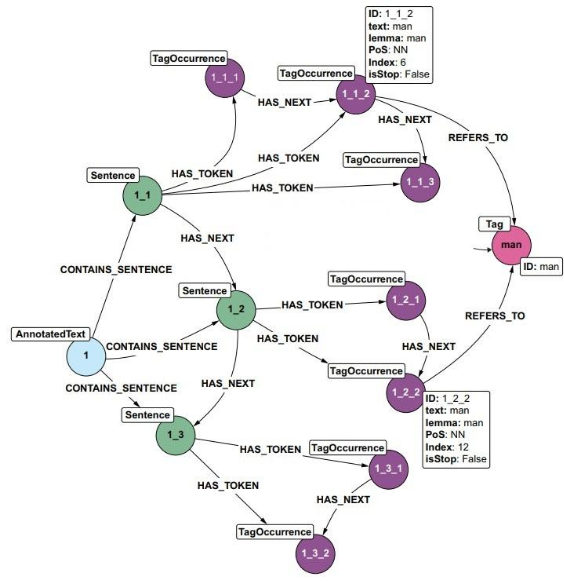
\includegraphics[width=0.5\linewidth]{RecommendationsGraph//img/graphfornlp.png}
\end{figure}
\\
Di conseguenza, con uno sforzo relativamente minimo, possiamo soddisfare il caso d'uso del \textbf{suggerimento di parole}, così come esigenze di \textbf{ricerca più complesse} e persino la \textbf{risposta a domande} (\textit{``Come sono le mele?''}).


